%%=============================================================================
%% Inleiding
%%=============================================================================

\chapter{Inleiding}
\label{ch:inleiding}

Sinds het grote succes van \textit{Bitcoin} is ``blockchain'' een vaste term geworden in het lexicon van de IT'er. Wat voor velen niet meer is dan een buzzwoord omtrent \textit{cryptogeld}, is voor anderen een trigger om te innoveren.
Die drang tot innovatie zet mensen ertoe aan om de technologie vanuit allerlei frisse invalshoeken te benaderen. Zodoende werd het toepassingsgebied van blockchain steeds uitgebreider, een proces dat nog volop aan de gang is. Ondernemers stellen zich de vraag of blockchain een meerwaarde kan bieden aan hun bedrijfsproces.

\section{Context}
\label{sec:context}

De insteek voor dit onderzoek kwam vanuit het softwarebedrijf 14IT. 14IT begon in 2014 met de ontwikkeling van CPSolution: een ERP-systeem door/voor kmo's. Een deel van het takenpakket bestaat uit het onderhouden en verder ontwikkelen van deze software. Binnen dit kader van \textit{continuous improvement} ontstond de interesse in dit onderwerp. Mede-eigenaar en copromotor Geert Borloo stelt zich de vraag of het programma verbeterd of uitgebreid kan worden door in te zetten op blockchaintechnologie. Vooral voor de dataopslag van facturen, contracten, abonnementen, ...  is 14IT benieuwd naar een mogelijke meerwaarde. Van hieruit ontstond de nood aan een onderzoek naar een mogelijke synergie tussen blockchain en ERP. 

\pagebreak

De doelstelling, zoals hierboven beschreven, kan herleid worden naar volgende onderzoeksvraag:

\begin{center}
	\textit{\textbf{``Hoe kunnen softwareontwikkelaars overgaan tot integratie van blockchaintechnologie voor de dataopslag van een ERP-systeem?''}}
\end{center}

In Hoofdstuk~\ref{ch:methodologie} -- \nameref{ch:methodologie} staat beschreven hoe deze onderzoeksvraag op hun systematische manier werd beantwoord.



\section{Verantwoording}
\label{sec:verantwoording}

Opkomende technologieën vormen wel vaker de insteek van nieuwe projecten en onderzoeken. Een eerste doorbraak spreekt tot de verbeelding en zet aan tot innovatie. Op die manier kunnen echte hypes ontstaan, zoals bij blockchain het geval is. Dat maakt het nog belangrijker om het onderzoeksgebied van deze bachelorproef doelgericht af te bakenen. Uit analyses van Gartner blijkt namelijk dat het potentieel van hypetechnologieën gemakkelijk overschat wordt~\autocite{Kietzmann2018}. Een succesvol onderzoek slaagt erin om hype te onderscheiden van mogelijks rendabele toepassingen.

\begin{figure}[H]
	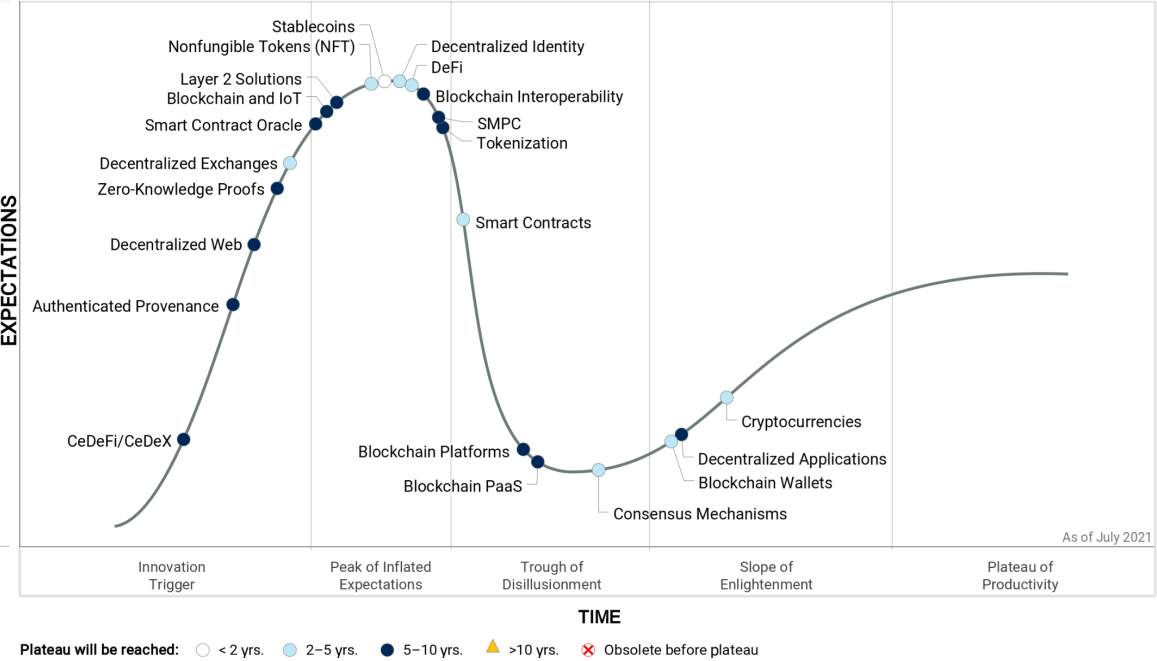
\includegraphics[width=\textwidth]{img/inleiding/gartner-hypecycle.png}
	\caption{\label{fig:gartner}Hype Cycle for Blockchain~\autocite{Gartner2021}}
\end{figure}

\pagebreak

In Figuur~\ref{fig:gartner} werd blockchain opgesplitst in 22 verschillende toepassingen. Elke toepassing werd voorgesteld als een punt op de Gartner Hype Cycle: een curve die weergeeft hoe de perceptie rond een hypetechnologie evolueert doorheen vijf vaste fases. Elk punt toont aan in welke fase de bijhorende toepassing zich bevindt (x-as) en als gevolg ook hoe hoog de verwachtingen errond zijn (y-as). De kleur van het punt stelt tevens een inschatting voor van hoe snel die toepassing matuur zal worden. 

Merk op dat 9 van de 22 toepassingen zich nog in de eerste opwaartse trend van de curve bevinden.
Die stijging wordt op gang getrokken door  een ``Innovation Trigger'' zoals een \textit{proof of concept} of belangstelling in de media. Men schat het potentieel heel hoog in, hoewel daar op dat moment nog weinig tot niets van in vervulling gebracht is. Hierdoor bereiken de verwachtingen al snel een maximum dat aanzienlijk hoger ligt dan wat de toepassing daadwerkelijk zal kunnen waarmaken: de ``Peak of Inflated Expectations''. Deze schromelijke overschatting zorgt gelukkig wel voor het nodige initiatief om de eerste commerciële projecten op poten te zetten. Een proces dat nog heel riskant is in dit ontwikkelingsstadium.

De ``Trough of Disillusionment'' maakt zijn intrede wanneer de eerste projecten niet het gewenste resultaat opleveren.
De verwachtingen van investeerders gaan de dieperik in door wat voor hen overkomt als mislukte experimenten. Desondanks is het een fase die zich aanbiedt als de geschikte gelegenheid tot onderzoek. Toepassingen, zoals ``Smart Contracts'' en ``Blockchain Platforms (aaS)'' komen stilaan \textit{down to earth} en vallen daarom mooi binnen de scope van deze paper. Een mix van succesverhalen en mislukkingen zorgen ervoor dat de grootste waanbeelden de deur uit zijn. De eerste commerciële implementaties doen hun intrede op de markt. Ze staan weliswaar nog in hun kinderschoenen, waardoor de vraag uit Sectie~\ref{sec:context} -- \nameref{sec:context} echt wel als een onderzoeksvraag mag beschouwd worden. 

In de huidige fase is het nog moeilijk om te beslissen of er mee op de trein gesprongen moet worden of niet. Met dit onderzoek kan hopelijk al een voorproefje gevonden worden van wat de ``Slope of Enlightenment'' zal brengen. Op die manier kan blockchain al benut worden voor de voordelen die binnen enkele jaren pas glashelder zullen worden. De ``Plateau of Productivity'' zal pas bereikt worden wanneer mainstream implementaties algemeen benut worden.

\newpage

\section{Opzet van deze bachelorproef}
\label{sec:opzet-van-deze-bachelorproef}

% Het is gebruikelijk aan het einde van de inleiding een overzicht te
% geven van de opbouw van de rest van de tekst. Deze sectie bevat al een aanzet
% die je kan aanvullen/aanpassen in functie van je eigen tekst.

De doelstelling van deze bachelorproef is om na te gaan of er een plaats is voor blockchain binnen het ERP-systeem van 14IT. Het is niet meteen duidelijk of het al dan niet haalbaar is voor kmo's om data op te slaan in een blockchain. Daarnaast blijft ook nog de vraag of hier nuttige \textit{use cases} voor weggelegd zijn. Om het onderzoek te laten slagen, was het van cruciaal belang om een resultaat na te streven dat praktisch bruikbaar is door 14IT. Dat gebeurde op twee manieren. 

Enerzijds moet dit werkstuk de lezer in staat stellen om zich op een vlotte manier in te werken in het onderwerp. Er valt al veel informatie te vinden over blockchains, waarvan niet alles even interessant is voor een ERP-systeem. De opbouw die in deze bachelorproef werd nagestreefd, zou 14IT moeten helpen om de state-of-the-art van het onderwerp snel te vatten.

Anderzijds biedt deze bachelorproef een \textit{proof of concept}. Deze zet de kennis en bevindingen van de sciptie om in een concrete toepassing. Het geeft 14IT een duidelijk beeld van wat mogelijk is binnen hun softwarepakket.

